\documentclass[12pt]{article}

% Packages
\usepackage[utf8]{inputenc}
\usepackage[T1]{fontenc}
\usepackage{amsmath}
\usepackage{amsfonts}
\usepackage{amssymb}
\usepackage{graphicx}
\usepackage{geometry}
\usepackage{float}
\usepackage{caption}
\usepackage{subcaption}
\usepackage{hyperref}
\usepackage{cite}
\usepackage{listings}
\usepackage{xcolor}
\usepackage{booktabs}
\usepackage{multirow}
\usepackage{enumitem}

% Page setup
\geometry{
    letterpaper,
    margin=1in,
    top=1in,
    bottom=1in
}

% Hyperlink setup
\hypersetup{
    colorlinks=true,
    linkcolor=blue,
    filecolor=magenta,      
    urlcolor=cyan,
    citecolor=red
}

% Code listing setup
\lstset{
    basicstyle=\ttfamily\small,
    keywordstyle=\color{blue},
    commentstyle=\color{gray},
    stringstyle=\color{red},
    numbers=left,
    numberstyle=\tiny,
    stepnumber=1,
    numbersep=5pt,
    backgroundcolor=\color{gray!10},
    showspaces=false,
    showstringspaces=false,
    showtabs=false,
    frame=single,
    tabsize=2,
    captionpos=b,
    breaklines=true,
    breakatwhitespace=false,
    escapeinside={\%*}{*)}
}

% Title page information
\title{Progress Report 1 : Miniature Tabletop Greenhouse Mechanism}
\author{Peyton Lettau, Sebastian Hondl, John Robinson, Will McConnell}
\date{\today}

\begin{document}

% Title page
\maketitle

% Abstract
\begin{abstract}
This report presents the analysis and design of advanced mechanisms for [project description]. The work includes type synthesis, kinematic analysis, and optimization of mechanical systems. Key findings and contributions are summarized in this abstract.
\end{abstract}

% Table of contents
\tableofcontents
\newpage

% Main content sections
\section{Introduction}
\label{sec:introduction}

A greenhouse creates a controlled microclimate by admitting short-wave solar radiation while slowing heat loss, raising temperature and humidity to support plant growth. Core requirements include high light transmission, thermal retention, and moisture control, balanced with sufficient ventilation to prevent overheating. In miniature formats (desktop or bench-scale), these same principles are compressed to a smaller area, but certain criteria become more difficult to maintain due to scaling effects.

\subsection{Background}
\label{sec:background}

In miniature greenhouses, low thermal mass causes rapid temperature swings, condensation accumulates quickly, and airflow pathways are easily blocked by foliage. These new challenges require the greenhouse access and function to be re-designed to allow full, unrestricted access and ventilation without disturbing the plants.

Common access solutions range from simple to engineered approaches. Low-tech options include cloches and cold-frame-style hinged lids, sliding or lift-off clear panels, roll-up soft sides, zipper covers, and magnetic or hook-and-loop closures. More refined mechanisms add hold-open features and controllable venting: front-hinged or top-hinged lids with friction hinges or gas springs; scissor-link or four-bar "pop-top" lids that lift and translate to clear the aperture; rack-and-pinion or cam-assisted lift for precise positioning; and side-access tambour doors for tight spaces. Many designs integrate passive vents or adjustable slots to decouple "brief access" from "continuous airflow," plus drip-management features to keep condensate off plants and electronics.

For a miniature unit, desirable traits include one-hand operation, stable hold-open, minimal visual obstruction, easy cleaning, and manufacturability. The challenge lies in adapting full-scale greenhouse mechanisms to small-scale applications, where existing solutions face significant limitations.

\subsubsection{Existing Patent Analysis}
\label{sec:patent_analysis}

While numerous full-scale greenhouse designs exist that use mechanisms to open and close plant barriers, small-scale greenhouses and terrariums typically rely on tiny components that become tedious to operate due to their size. The improvements sought for this project involve developing mechanisms specifically suited for small-scale applications that are not currently available on the market.

\textbf{Patent 1 - Portable Greenhouse (\cite{Koziol1974}):} This patent represents a practical full-scale greenhouse solution using a different opening and closing system. While effective at full size, scaling this design down presents significant operational challenges. The plurality of covered sides becomes more complex to operate when the greenhouse is positioned on a desk, and the mechanism components become proportionally smaller and more difficult to manipulate.

\textbf{Patent 2 - Full-Scale Greenhouse Covering (\cite{Jaderloon1999}):} This design functions to keep out rainwater using cable systems, rotating shafts, and tension drums that require very precise alignment. While effective at full scale, these systems are not feasible for small-scale applications. Scaling down would make parts more fragile, expensive, and difficult to assemble. Additionally, the tension in cables does not scale proportionally when reduced to smaller sizes, leading to inadequate performance or excessive complexity.

\textbf{Patent 3 - Greenhouse Window Mechanism (\cite{Bom1978}):} This patent shows an opening and closing mechanism for greenhouse windows that demonstrates potential scalability to the current project. The mechanism relies on rigid bars and rotational joints, making it more suitable for adaptation to small-scale applications. The triangular guide-bar linkage coordinates multiple vents with stable geometry, offering promise for synchronized, multi-panel tabletop access.

The analysis of these patents reveals that while full-scale greenhouse mechanisms exist, there is a clear gap in the market for small-scale mechanisms that maintain the functionality and reliability of their larger counterparts while being appropriately sized and proportioned for desktop applications.

\section{Goals Statement}
Design and build a compact mechanism that opens and closes a tabletop greenhouse whose sides are constrained by adjacent walls/edges—no linkages may sweep outside the footprint. The mechanism shall articulate the top and front panels to provide full, unobstructed plant access and offer stable, adjustable hold-positions along the motion path for customizable ventilation.

\section{Task Specification}
The challenge is to design a six-bar linkage mechanism that enables controlled, simultaneous opening of both the top and front panels of a tabletop greenhouse while satisfying multiple engineering constraints and performance requirements.

\begin{itemize}
    \item Provide smooth, controlled motion for fragile glass panels (1/8" thick)
    \item Enable access to plants from both top and front faces simultaneously
    \item Operate within compact tabletop dimensions (approximately 18" tall × 18" deep × 24" wide)
    \item Incorporate spring balancing to reduce actuation forces and prevent impact damage
    \item The opening above the enclosure must be >90\% of the depth of the enclosure
    \item Mechanism must not extend beyond the greenhouse silhouette when closed
    \item Compatible with placement against a wall
    \item Minimize interference with internal plant growth space
    \item Allow front and top of the enclosure to be positioned at any position between open and close and remain in place
    \item Fold the top and front panels above the enclosure, creating unobstructed access for plant maintenance
    \item Optimize linkage geometry to provide smooth velocity profiles while maintaining mechanical advantage throughout the operating range
    \item Support the weight of the front and top of the enclosure ( ~ 5lb each)
\end{itemize}


\section{Methodology}
\label{sec:methodology}

\subsection{Type Synthesis Process}
\label{sec:type_synthesis}

Type synthesis was conducted following the systematic methodology outlined by Erdman \& Mather (2024) to identify the optimal mechanism topology for the tabletop greenhouse application before proceeding to dimensional synthesis. Applying Gruebler's equation for planar mechanisms, $F = 3(n-1) - 2f_1 - f_2$, with the requirement of single-degree-of-freedom motion ($F=1$) and using only revolute joints ($f_2=0$), we initially evaluated four-bar mechanisms where $n=4$ yields $f_1=4$. However, initial synthesis attempts demonstrated that four-bar linkages cannot simultaneously satisfy the spatial constraints—ground pivots must be located at the base within 8 cm height with maximum 25 cm separation—and achieve the required door motion of 0° to 45° rotation with translation through three precision positions. The compact greenhouse envelope (30 cm × 30 cm × 30 cm) combined with ground pivot placement restrictions resulted in no feasible four-bar solutions. This analysis necessitated exploration of six-bar mechanisms ($n=6$), which require $f_1=7$ revolute joints and provide greater design flexibility through two independent kinematic loops.

Using the equation $n-(F+3)=T+2Q+3P$ to determine link types, where $T$, $Q$, and $P$ represent ternary, quaternary, and pentagonal links respectively, we find that $6-(1+3)=2$ for our six-bar, single-DOF mechanism. The standard kinematic link set solution (KLSS) comprises 2 ternary links and 4 binary links, providing the foundation for mechanism topology development. Systematic enumeration of basic kinematic chains (BKCs) from this KLSS, with application of the degree-of-freedom distribution criterion to eliminate configurations containing zero-freedom subchains, yields two valid BKCs: the Watt chain, characterized by two ternary links sharing a common connection, and the Stephenson chain, where the ternary links are separated by binary links. These two fundamental topologies form the basis for all six-bar, single-DOF mechanisms with revolute joints.

\begin{figure}[H]
    \centering
    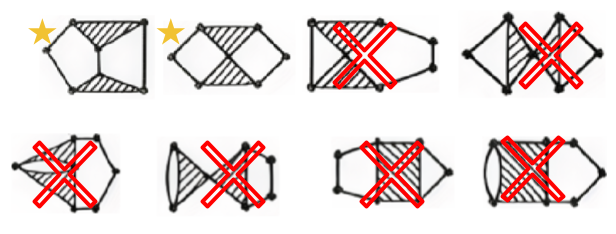
\includegraphics[width=0.8\textwidth]{6 Bar options.png}
    \caption{Six-bar mechanism topology options}
    \label{fig:six_bar_options}
\end{figure}

Grounding different links within each BKC through kinematic inversion produces five unique topological variations: Watt I, Watt II, Stephenson I, Stephenson II, and Stephenson III. Each inversion was systematically evaluated against design-specific criteria following the approach demonstrated in the Type Synthesis Handout. The critical differentiator proved to be ground pivot accessibility: Watt II, Stephenson II, and Stephenson III all require ternary ground links with three ground pivots, which cannot be practically accommodated on the compact greenhouse base structure without interfering with the interior growing space or requiring pivots at incompatible heights. Stephenson I, while featuring only two ground pivots, exhibits an extended structure with separated ternary links that results in longer link lengths and potentially unfavorable transmission angles for this application.

\begin{figure}[H]
    \centering
    \includegraphics[width=0.8\textwidth]{stephenson and watt.png}
    \caption{Stephenson and Watt chain configurations with kinematic inversions}
    \label{fig:stephenson_watt}
\end{figure}

The Watt I configuration emerged as the optimal topology, uniquely satisfying all requirements with its binary ground link providing two accessible ground pivots positioned at the front base edge (15-20 cm separation), compact dual-loop structure enabling link lengths of 8-20 cm within the spatial envelope, and favorable transmission angle characteristics throughout the anticipated range of motion. All seven joints are specified as revolute (pin) joints for manufacturing simplicity and cost-effectiveness. While transformation laws permit substitution of prismatic joints for revolute joints or incorporation of higher pairs such as gears or cams, such modifications offer no functional advantage for this low-speed greenhouse application and would increase fabrication complexity. The selected configuration positions the binary link connected to ground pivot $G_A$ as the input crank, accessible for external user interaction while the mechanism guides the door panel through the three precision positions: closed (0°), ventilation (~30°), and fully open (~45°). This systematic type synthesis process ensures that subsequent dimensional synthesis efforts focus on a topology with proven spatial compatibility and kinematic suitability for the greenhouse application.

\subsection{Kinematic Analysis}
[Add kinematic analysis methods]

\section{Results and Analysis}
\label{sec:results}

\subsection{Solution Progress}
\label{sec:solution_progress}

Initial work towards a solution focused primarily on finding a four-bar linkage for path generation. This approach has not been successful in meeting the design requirements. The "best" solution obtained thus far fails to satisfy the spatial constraints, as the mechanism extends beyond the front edge of the enclosure in the closed position. Additionally, the force analysis reveals extremely high joint and link forces due to the mechanical disadvantage created by the short distance between the upper and lower link connections to the coupler compared to the distance between these joints and the front panel attachment point.

This solution and numerous alternatives were synthesized using MATLAB's MultiStart optimization algorithm to identify configurations that pass through or near multiple precision positions while attempting to satisfy spatial constraints. Multiple iterations were attempted using various precision position sets and different quantities of precision positions, but none yielded satisfactory results within the four-bar framework.

\subsection{Solution Approach Options}
\label{sec:approach_options}

The design problem can be formulated through multiple approaches, each offering distinct advantages and challenges:

\begin{enumerate}
    \item \textbf{Path Generation}: A point on the front panel is selected as the coupler point, and a linkage is synthesized to guide this point through a series of precision positions while maintaining the front panel attachment through a pivot connection.
    
    \item \textbf{Motion Synthesis}: The top and front panels are linked within the mechanism, and the mechanism is synthesized based on the angular and positional relationships of the front panel throughout its range of motion.
    
    \item \textbf{Function Generation}: This approach requires a perspective shift where the top panel serves as the ground link, the main enclosure frame as the input link, and the front panel as the output link.
    
    \item \textbf{Combined Function and Motion Generation}: In this formulation, the top and front panels are not directly connected by a pin joint. Instead, the front panel is solely constrained by the mechanism, which simultaneously acts as a function generator to control the top panel motion as the front panel moves through its range of positions.
\end{enumerate}

\subsection{Selected Solution Approach}
\label{sec:selected_approach}

For this project, the path generation approach was selected as the primary design methodology. Initial work attempted to synthesize a four-bar linkage for this task, but analysis indicates that a satisfactory four-bar solution is unlikely to exist within the given constraints. However, it appears probable that an effective solution can be achieved using linkages with additional degrees of freedom, such as six-bar or eight-bar mechanisms.

\subsection{Design Process}
\label{sec:design_process}

The design process began with the fundamental requirement for single-degree-of-freedom motion with a single user input. The input mechanism consists solely of the user pulling upward on the door handle, with the entire door mechanism moving as a unified system through its complete range of motion to the fully opened position. This constraint establishes the requirement for one degree of freedom and one input link.

Initial mechanism design efforts focused on four-bar linkages, but analysis quickly revealed the impossibility of satisfying spatial constraints while achieving the required motion for the lower right-hand corner pivot location. The investigation then progressed to six-bar mechanisms, where two of the links would represent the top and front panels of the greenhouse. However, after preliminary sketches and motion analysis, an eight-bar mechanism was determined to offer superior performance characteristics.

Rather than attempting to design an eight-bar mechanism with two fixed-length links and ground pivots, the decision was made to pursue a six-bar path generation approach connected to the path of the lower right-hand pivot. This approach was selected based on the principle that additional links between the ground and control point provide more design variables, thereby increasing the likelihood of achieving the desired motion characteristics.

After comprehensive analysis and evaluation of different six-bar mechanism configurations, the Watt I mechanism was identified as the optimal topology for path generation. This selection is based on the principle that increased link complexity between the ground and control point enhances the feasibility of achieving the desired linkage performance through additional design variables.

\section{Future Work}
\label{sec:future}

[Add future work recommendations]

% References
\bibliographystyle{ieeetr}
\bibliography{references}

\cite{Bom1978}
\cite{Jaderloon1999}
\cite{Koziol1974}

% Appendices
\appendix



\end{document}

